\chapter{Termodinâmica estatística: funções de partição}\label{ch:b3:partition-functions}

O túmulo de Ludwig Boltzmann, em Viena, traz uma única linha, $S = k\log W$: a
entropia de um sistema conta as maneiras pelas quais suas moléculas podem
repartir sua energia. A termodinâmica, tal como os volumes do 1.º e do 2.º ano
a construíram, nunca precisa de moléculas: ela relaciona entre si calores,
entropias e constantes de equilíbrio medidos. A termodinâmica estatística os
calcula a partir das próprias moléculas. Seu objeto central é uma única soma
sobre os níveis de energia de uma molécula, a função de partição; os níveis
vêm da espectroscopia, e a entropia padrão do nitrogênio calculada a partir de
seu espectro concorda com o valor tabelado a um centésimo de joule por kelvin
e por mol. Este capítulo constrói a função de partição, decompõe-na em suas
partes translacional, rotacional, vibracional e eletrônica, e a transforma em
energia interna, entropia e energia de Gibbs; o
\cref{ch:b3:statistical-thermo-applied} a aplica às capacidades caloríficas e
às constantes de equilíbrio.

\begin{recall}
O volume do 2.º ano definiu a entropia molar padrão, a energia de Gibbs e o
potencial químico, e tabelou entropias obtidas a partir de capacidades
caloríficas medidas até baixas temperaturas. O \cref{ch:b3:quantum-model-systems}
deu os níveis de energia de uma \omterm{def:b3:quantum-model-systems:box}{partícula na caixa}, do \omterm{def:b3:quantum-model-systems:oscillator}{oscilador harmônico} e do
\omterm{def:b3:quantum-model-systems:rotor}{rotor rígido}, $E_J = hcBJ(J+1)$ com \omterm{def:b3:quantum-model-systems:degenerate}{degenerescência} $2J + 1$; o
\cref{ch:b3:rovibrational-spectroscopy} mediu $B$ e $\tilde\nu$ para moléculas
diatômicas e constatou que, em uma molécula homonuclear como \ce{N2}, os spins
nucleares tornam desiguais os níveis rotacionais alternados.
\end{recall}

\section{Microestados e a distribuição de Boltzmann}

Considere $N$ moléculas idênticas e independentes que podem ocupar níveis de
energia $\varepsilon_0 = 0 < \varepsilon_1 < \varepsilon_2 < \dots$, com energia total $E$. Dizer
quantas moléculas estão em cada nível, $\{n_0, n_1, \dots\}$, descreve uma
distribuição; dizer qual molécula está em qual nível descreve muito mais.

\begin{definition}[Microestado, peso estatístico]\label{def:b3:partition-functions:microstate}
Um \emph{microestado}\index{microestado} de um sistema de moléculas é uma
especificação completa do estado de cada molécula. O \emph{peso
estatístico}\index{peso estatistico@peso estatístico} $W$ de uma distribuição $\{n_i\}$ de $N$
moléculas sobre níveis não degenerados é o número de microestados que a realizam:
\[
  W = \frac{N!}{n_0!\,n_1!\,n_2!\cdots}.
\]
\end{definition}

\begin{example}[Três quanta entre três osciladores]\label{ex:b3:partition-functions:three-quanta}
Três osciladores compartilham três quanta de energia. A distribuição ``um
oscilador detém os três'' pode ser realizada de $3!/(1!\,2!) = 3$ maneiras, ``um
detém dois, outro um'' de $3! = 6$ maneiras e ``cada um detém um'' de uma
maneira: dez \omterm{def:b3:partition-functions:microstate}{microestados} ao todo, e a distribuição mais equilibrada que ainda
espalha a energia por vários níveis é a mais provável. Com $10^{23}$ moléculas,
os pesos ficam tão concentrados que uma distribuição, e as que diferem dela de
uma quantidade desprezível, reúnem praticamente todos os \omterm{def:b3:partition-functions:microstate}{microestados}.
\end{example}

\begin{remark}
O postulado da termodinâmica estatística é que todos os \omterm{def:b3:partition-functions:microstate}{microestados} de um
sistema isolado com uma dada energia são igualmente prováveis. O sistema é então
encontrado, de modo esmagador, na distribuição de maior peso: encontrá-la é a
tarefa desta seção.
\end{remark}

Para números grandes, a aproximação de Stirling $\ln x! \approx x\ln x - x$ dá
\[
  \ln W = N\ln N - \sum_i n_i\ln n_i .
\]

\begin{definition}[Distribuição de Boltzmann, população]\label{def:b3:partition-functions:boltzmann}
A \emph{população}\index{populacao@população} $n_i/N$ de um nível é a fração das
moléculas que o ocupam. A \emph{distribuição de Boltzmann}\index{distribuicao de Boltzmann@distribuição de Boltzmann}
é a distribuição de maior peso de moléculas independentes em
equilíbrio térmico à temperatura $T$, dada pelo teorema abaixo.
\end{definition}

\begin{theorem}[A distribuição de Boltzmann]\label{thm:b3:partition-functions:boltzmann}
Para moléculas independentes em equilíbrio à temperatura $T$, a \omterm{def:b3:partition-functions:boltzmann}{população} de um
nível de energia $\varepsilon_i$ e \omterm{def:b3:quantum-model-systems:degenerate}{degenerescência} $g_i$ é
\[
  \frac{n_i}{N} = \frac{g_i\eu^{-\varepsilon_i/kT}}{q},
  \qquad q = \sum_i g_i\eu^{-\varepsilon_i/kT},
\]
onde $k$ é a constante de Boltzmann. Dois níveis têm \omterm{def:b3:partition-functions:boltzmann}{populações} na razão
$\frac{n_j}{n_i} = \frac{g_j}{g_i}\eu^{-(\varepsilon_j - \varepsilon_i)/kT}$.
\end{theorem}

\begin{proof}[Demonstração parcial]
Tome primeiro níveis não degenerados. Maximize $\ln W$ sob as duas restrições
$\sum_in_i = N$ e $\sum_in_i\varepsilon_i = E$ com os multiplicadores de Lagrange $\alpha$ e $\beta$:
para todo $i$,
\[
  \frac{\partial}{\partial n_i}\Bigl(\ln W + \alpha\sum_jn_j - \beta\sum_jn_j\varepsilon_j\Bigr)
  = -\ln n_i - 1 + \alpha - \beta\varepsilon_i = 0,
\]
logo $n_i = \eu^{\alpha - 1}\eu^{-\beta\varepsilon_i}$, e a primeira restrição fixa $\eu^{\alpha - 1}
= N/\sum_j\eu^{-\beta\varepsilon_j}$. Um nível de \omterm{def:b3:quantum-model-systems:degenerate}{degenerescência} $g_i$ são $g_i$ estados distintos de
mesma energia, cada um povoado como acima: sua \omterm{def:b3:partition-functions:boltzmann}{população} é multiplicada por
$g_i$. O multiplicador $\beta$ é identificado por um caso conhecido: para o
movimento de translação de um gás ideal (\cref{prop:b3:partition-functions:q-trans}
adiante), a distribuição dá uma energia $\frac32N/\beta$, e a energia do gás
ideal é $\frac32NkT$; logo $\beta = 1/kT$. Que $\beta$ seja a mesma grandeza para todo
tipo de movimento, e que ela seja a temperatura termodinâmica, é admitido
aqui: dois sistemas em contato térmico compartilham o mesmo $\beta$, o que é a
propriedade que define a temperatura.
\end{proof}

\begin{definition}[Função de partição molecular]\label{def:b3:partition-functions:partition-function}
A \emph{função de partição molecular}\index{funcao de particao molecular@função de partição molecular} de uma
molécula à temperatura $T$ é a soma
\[
  q = \sum_{\text{níveis}}g_i\eu^{-\varepsilon_i/kT} = \sum_{\text{estados}}\eu^{-\varepsilon_s/kT},
\]
com as energias medidas a partir do nível mais baixo, de modo que $q \ge 1$.
\end{definition}

A função de partição conta os estados termicamente acessíveis: a temperatura
muito baixa, só o nível mais baixo contribui e $q \to g_0$; a temperatura muito
alta, cada estado contribui com cerca de 1 e $q$ cresce sem limite. Daí uma
regra prática: os níveis situados muito mais de $kT$ acima do mais baixo estão
vazios, os níveis a menos de $kT$ dele estão povoados. A \qty{298.15}{K}, $kT$
corresponde a \qty{207.2}{cm^{-1}}, ou $RT = \qty{2.479}{kJ/mol}$.

\begin{method}[Populações dos níveis a partir das constantes espectroscópicas]\label{met:b3:partition-functions:populations}
\begin{enumerate}
  \item Liste os níveis com suas energias (a partir das constantes, por exemplo
        $hcBJ(J+1)$) e \omterm{def:b3:quantum-model-systems:degenerate}{degenerescências} ($2J + 1$).
  \item Exprima cada energia em unidades de $kT$; a \qty{298.15}{K}, divida um
        número de onda por \qty{207.2}{cm^{-1}}.
  \item Forme os termos $g_i\eu^{-\varepsilon_i/kT}$, some-os para obter $q$ e divida.
        Interrompa a soma quando os termos forem desprezíveis.
  \item Verifique: as \omterm{def:b3:partition-functions:boltzmann}{populações} somam 1; a razão entre duas delas é
        $\frac{g_j}{g_i}\eu^{-(\varepsilon_j-\varepsilon_i)/kT}$.
\end{enumerate}
\end{method}

\begin{example}[Os níveis rotacionais do cloreto de hidrogênio]\label{ex:b3:partition-functions:hcl}
% ledger: diat:HCl.Be, diat:HCl.ae
Para \ce{H^{35}Cl}, $B_0 = B_e - \alpha_e/2 = \qty{10.44}{cm^{-1}}$. A \qty{300}{K}, o nível $J$
fica em $10.44\,J(J+1)$~\unit{cm^{-1}}, isto é, $0.0501\,J(J+1)$ em unidades de $kT$. Os termos
$(2J+1)\eu^{-0.0501J(J+1)}$ valem 1, 2.71, 3.70, 3.84, 3.31, 2.45, \dots; sua soma é
$q = 20.3$, e as \omterm{def:b3:partition-functions:boltzmann}{populações} de $J = 0$ a 4 são 0.049, 0.134, 0.182, 0.189 e
0.163: o nível mais povoado é $J = 3$, e não $J = 0$, porque a \omterm{def:b3:quantum-model-systems:degenerate}{degenerescência}
$2J + 1$ cresce enquanto o fator de Boltzmann diminui. É a envoltória da
banda de rotação--vibração do \cref{ch:b3:rovibrational-spectroscopy}.
\end{example}

\begin{omfigure}
\begin{tikzpicture}[font=\small]
  % levels J = 0-3, g = 2J+1, energies 0, 1, 3, 6 (units of 2hcB); bars = 3.5 cm x population
  % of the four levels alone at kT = 2hcB (0.422, 0.466, 0.105, 0.007) and kT = 10hcB (0.120, 0.296, 0.330, 0.254)
  \foreach \J/\e/\g/\lo/\hi in {0/0/1/1.48/0.42, 1/1/3/1.63/1.04, 2/3/5/0.37/1.16, 3/6/7/0.03/0.89}{
    \draw[thick] (0,0.55*\e) -- (2.2,0.55*\e);
    \node[anchor=east] at (0,0.55*\e) {$J = \J$};
    \node[anchor=west, font=\scriptsize] at (2.25,0.55*\e) {$g = \g$};
    \fill[omDef!70] (3.4,0.55*\e-0.11) rectangle ++(\lo,0.22);
    \fill[omThm!70] (6.4,0.55*\e-0.11) rectangle ++(\hi,0.22);
  }
  \node[anchor=south, omDef] at (4.2,3.6) {$T$ baixa};
  \node[anchor=south, omThm] at (7.2,3.6) {$T$ alta};
  \draw[->] (-1.4,0) -- (-1.4,3.7) node[anchor=south] {$\varepsilon$};
\end{tikzpicture}

{\small Uma escada de Boltzmann: níveis rotacionais $J = 0$ a 3 (energias $0$, $2$, $6$,
$12$ vezes $hcB$, \omterm{def:b3:quantum-model-systems:degenerate}{degenerescências} $2J + 1$) e suas \omterm{def:b3:partition-functions:boltzmann}{populações}, como comprimentos de
barra, a $kT = 2hcB$ e a $kT = 10hcB$ (somente os quatro níveis). O aquecimento esvazia
o nível mais baixo em proveito dos superiores; nas duas temperaturas, as barras somam
o mesmo total, o número de moléculas.}
\end{omfigure}

\section{A função de partição molecular}

\begin{proposition}[Fatoração]\label{prop:b3:partition-functions:factorisation}
Se a energia de uma molécula é uma soma de contribuições independentes,
$\varepsilon = \varepsilon^{\mathrm T} + \varepsilon^{\mathrm R} + \varepsilon^{\mathrm V} + \varepsilon^{\mathrm E}$, sendo cada estado
uma combinação qualquer de um estado translacional, um rotacional, um vibracional
e um eletrônico, então
\[
  q = q^{\mathrm T}q^{\mathrm R}q^{\mathrm V}q^{\mathrm E}.
\]
\end{proposition}

\begin{proof}
A soma sobre todas as combinações da exponencial de uma soma é o produto das
somas separadas: $\sum_{a,b}\eu^{-(\varepsilon_a+\varepsilon_b)/kT} = \bigl(\sum_a\eu^{-\varepsilon_a/kT}\bigr)
\bigl(\sum_b\eu^{-\varepsilon_b/kT}\bigr)$, e o mesmo para quatro fatores.
\end{proof}

A separação é uma aproximação: rotação e vibração interagem (a constante
$\alpha_e$), e o estado eletrônico fixa as \omterm{def:b3:rovibrational-spectroscopy:rotational-constant}{constantes rotacionais} e
vibracionais. Para uma molécula em seu estado eletrônico fundamental a
temperaturas usuais, os erros são de alguns centésimos de joule por kelvin em
uma entropia. As \omterm{def:b3:partition-functions:boltzmann}{populações} são então calculadas separadamente para cada tipo
de movimento: a fração de moléculas em um nível vibracional $v$ não depende de
sua rotação.

\section{As quatro contribuições}

\subsection*{Translação}

\begin{definition}[Comprimento de onda térmico]\label{def:b3:partition-functions:thermal-wavelength}
O \emph{comprimento de onda térmico}\index{comprimento de onda termico@comprimento de onda térmico} de uma molécula de massa $m$
à temperatura $T$ é $\Lambda = \dfrac{h}{\sqrt{2\pi mkT}}$.
\end{definition}

\begin{proposition}[Função de partição translacional]\label{prop:b3:partition-functions:q-trans}
Para uma molécula de massa $m$ livre para se mover em um volume $V$,
\[
  q^{\mathrm T} = \frac{V}{\Lambda^3}.
\]
\end{proposition}

\begin{proof}
Em uma dimensão, uma caixa de comprimento $L$ tem os níveis $\varepsilon_n = h^2n^2/8mL^2$
($n = 1, 2, \dots$; o deslocamento do ponto zero não altera nada mensurável). Eles
estão tão próximos que a soma é uma integral:
\[
  q_x = \sum_{n\ge1}\eu^{-h^2n^2/8mL^2kT} \approx \int_0^\infty\eu^{-h^2n^2/8mL^2kT}\dd n
      = \frac12\sqrt{\frac{\pi\,8mL^2kT}{h^2}} = \frac{L\sqrt{2\pi mkT}}{h} = \frac{L}{\Lambda}.
\]
As três direções são independentes: $q^{\mathrm T} = q_xq_yq_z = L^3/\Lambda^3$. A
energia média por dimensão é $-\partial\ln q_x/\partial\beta$ com $q_x \propto \beta^{-1/2}$, isto é,
$1/2\beta$; três dimensões dão $\frac32kT$ por molécula, como usado na demonstração do
\cref{thm:b3:partition-functions:boltzmann}.
\end{proof}

\begin{example}[Argônio em um frasco]\label{ex:b3:partition-functions:argon}
% ledger: aw:Ar, const:h, const:kB
Para o argônio ($M = \qty{39.95}{g/mol}$) a \qty{298.15}{K}, $\Lambda = \qty{16.0}{pm}$, um décimo
de um diâmetro atômico. Em \qty{1}{dm^3}, $q^{\mathrm T} = 10^{-3}/(1.600\times10^{-11})^3 = \num{2.44e29}$
estados translacionais estão termicamente acessíveis, muito mais que os
$2.4\times10^{22}$ átomos que o frasco contém a \qty{1}{bar}: cada estado está quase
sempre vazio, condição sob a qual as moléculas podem ser contadas como a seguir.
\end{example}

\subsection*{Rotação}

\begin{definition}[Temperaturas características]\label{def:b3:partition-functions:characteristic-temperature}
A \emph{temperatura característica de rotação}\index{temperatura caracteristica de rotacao@temperatura característica de rotação}
de uma molécula linear de \omterm{def:b3:rovibrational-spectroscopy:rotational-constant}{constante rotacional} $B$ é $\theta_{\mathrm R} =
hcB/k$; a \emph{temperatura característica de vibração}\index{temperatura caracteristica de vibracao@temperatura característica de vibração}
de uma vibração de número de onda $\tilde\nu$ é $\theta_{\mathrm V} =
hc\tilde\nu/k$.
\end{definition}

\begin{definition}[Número de simetria]\label{def:b3:partition-functions:symmetry-number}
O \emph{número de simetria}\index{numero de simetria@número de simetria} $\sigma$ de uma molécula é o
número de orientações distintas da molécula rígida que são alcançadas por
rotações próprias e são indistinguíveis da orientação de partida (a ordem do
\omterm{def:b3:point-groups:class}{subgrupo} de rotações de seu \omterm{def:b3:point-groups:point-group}{grupo pontual}): 1 para \ce{HCl} e \ce{CO}, 2 para \ce{N2},
\ce{CO2} e \ce{H2O}, 3 para \ce{NH3}, 12 para \ce{CH4} e \ce{C6H6}.
\end{definition}

\begin{proposition}[Função de partição rotacional]\label{prop:b3:partition-functions:q-rot}
Para uma molécula linear, $q^{\mathrm R} = \sum_J(2J+1)\eu^{-\theta_{\mathrm R}J(J+1)/T}$. Quando $T \gg
\theta_{\mathrm R}$,
\[
  q^{\mathrm R} \approx \frac{T}{\sigma\theta_{\mathrm R}} = \frac{kT}{\sigma hcB},
\]
com um erro relativo de cerca de $\theta_{\mathrm R}/3T$ para $\sigma = 1$ (a soma exata é próxima
de $T/\theta_{\mathrm R} + \frac13$).
\end{proposition}

\begin{proof}[Demonstração parcial]
Para $T \gg \theta_{\mathrm R}$, muitos níveis contribuem e a soma se torna uma integral.
Com $x = J(J+1)$, $\dd x = (2J+1)\dd J$:
\[
  \int_0^\infty(2J+1)\eu^{-\theta_{\mathrm R}J(J+1)/T}\dd J = \int_0^\infty\eu^{-\theta_{\mathrm R}x/T}\dd x
  = \frac{T}{\theta_{\mathrm R}}.
\]
A correção $\frac13$ vem do termo seguinte da fórmula de Euler--Maclaurin
(\cref{exo:b3:partition-functions:11}). O fator $1/\sigma$ é admitido aqui e
justificado no \cref{ch:b3:statistical-thermo-applied}: em uma molécula
homonuclear, a simetria da função de onda na permutação dos dois núcleos
idênticos só permite a cada estado de spin nuclear uma paridade de $J$
(\cref{ch:b3:rovibrational-spectroscopy}), de modo que, em média, metade dos
níveis rotacionais falta. Contar os estados rotacionais com $\sigma$ dessa maneira
deixa os estados de spin nuclear fora de $q$; as tabelas termodinâmicas seguem a
mesma convenção, e o fator de spin nuclear se cancela em toda reação química.
\end{proof}

Para \ce{N2}, $B_0 = \qty{1.990}{cm^{-1}}$ e $\theta_{\mathrm R} = \qty{2.86}{K}$: a \qty{298.15}{K},
$q^{\mathrm R} = 298.15/(2\times2.863) = 52.1$. Para \ce{HCl}, $\theta_{\mathrm R} = \qty{15.0}{K}$ e
$q^{\mathrm R} = 19.8$ (soma exata 20.2). Só o \ce{H2} ($\theta_{\mathrm R} = \qty{85}{K}$) e seus \omterm{def:b3:rovibrational-spectroscopy:rotational-constant}{isotopólogos}
precisam da soma exata à temperatura ambiente. Uma molécula não linear de \omterm{def:b3:rovibrational-spectroscopy:rotational-constant}{constantes
rotacionais} $A$, $B$, $C$ tem $q^{\mathrm R} = \frac{1}{\sigma}\bigl(\frac{kT}{hc}\bigr)^{3/2}\sqrt{\frac{\pi}{ABC}}$, admitido.

\subsection*{Vibração}

\begin{proposition}[Função de partição vibracional]\label{prop:b3:partition-functions:q-vib}
Para uma vibração harmônica de número de onda $\tilde\nu$, com as energias medidas a
partir do nível do ponto zero,
\[
  q^{\mathrm V} = \sum_{v\ge0}\eu^{-v\theta_{\mathrm V}/T} = \frac{1}{1 - \eu^{-\theta_{\mathrm V}/T}} .
\]
Ela tende a 1 quando $T \ll \theta_{\mathrm V}$ e a $T/\theta_{\mathrm V}$ quando $T \gg \theta_{\mathrm V}$. Uma molécula
com vários \omterm{def:b3:group-theory-applied:normal-mode}{modos normais} tem o produto de um fator desses por modo.
\end{proposition}

\begin{proof}
Os níveis ficam $v\,hc\tilde\nu$ acima do nível do ponto zero: a soma é uma série geométrica
de razão $\eu^{-\theta_{\mathrm V}/T} < 1$. Quando $T \gg \theta_{\mathrm V}$, $1 - \eu^{-\theta_{\mathrm V}/T} \approx \theta_{\mathrm V}/T$.
Os \omterm{def:b3:group-theory-applied:normal-mode}{modos normais} são independentes (\cref{prop:b3:partition-functions:factorisation}).
\end{proof}

Para o quantum vibracional de uma molécula diatômica, este livro toma a
fundamental observada $G(1) - G(0) = \omega_e - 2\omega_ex_e$
(\cref{ch:b3:rovibrational-spectroscopy}); à temperatura ambiente, só os primeiros
níveis importam, e é o seu espaçamento que conta. As moléculas rígidas e leves
estão congeladas: \ce{N2} tem $\theta_{\mathrm V} = \qty{3352}{K}$, $q^{\mathrm V} = 1.000013$ a \qty{298.15}{K}, e
apenas 13 moléculas em um milhão estão em $v = 1$. As pesadas e moles não estão: \ce{I2}
tem $\theta_{\mathrm V} = \qty{307}{K}$, $q^{\mathrm V} = 1.556$, e mais de um terço de suas moléculas
vibra.

\begin{omfigure}
\begin{tikzpicture}
\begin{axis}[name=rotA, width=0.36\linewidth, height=5.0cm, xmin=-0.5, xmax=14.5,
  ymin=0, ymax=0.34, axis lines=left, ycomb, xlabel={$J$}, ylabel={população},
  tick label style={font=\scriptsize}, label style={font=\small},
  title={\small \ce{HCl}, rotação}, scaled y ticks=false,
  yticklabel style={/pgf/number format/fixed}]
\addplot[omDef, line width=1.6pt, xshift=-1.6pt] table[x=J, y=T100] {figdata/out/bachelor-3-boltzmann-populations-hcl.dat};
\addplot[black!60, line width=1.6pt] table[x=J, y=T300] {figdata/out/bachelor-3-boltzmann-populations-hcl.dat};
\addplot[omThm, line width=1.6pt, xshift=1.6pt] table[x=J, y=T1000] {figdata/out/bachelor-3-boltzmann-populations-hcl.dat};
\end{axis}
\begin{axis}[name=rotB, at={(rotA.east)}, anchor=west, xshift=0.9cm, width=0.36\linewidth,
  height=5.0cm, xmin=-1, xmax=41, ymin=0, ymax=0.17, axis lines=left, ycomb,
  xlabel={$J$}, tick label style={font=\scriptsize}, label style={font=\small},
  title={\small \ce{CO}, rotação}, scaled y ticks=false,
  yticklabel style={/pgf/number format/fixed}]
\addplot[omDef, sharp plot, thin, mark=*, mark size=0.9pt] table[x=J, y=T100] {figdata/out/bachelor-3-boltzmann-populations-co.dat};
\addplot[black!60, sharp plot, thin, mark=*, mark size=0.9pt] table[x=J, y=T300] {figdata/out/bachelor-3-boltzmann-populations-co.dat};
\addplot[omThm, sharp plot, thin, mark=*, mark size=0.9pt] table[x=J, y=T1000] {figdata/out/bachelor-3-boltzmann-populations-co.dat};
\end{axis}
\begin{axis}[at={(rotB.east)}, anchor=west, xshift=0.9cm, width=0.32\linewidth,
  height=5.0cm, xmin=-0.5, xmax=10.5, ymin=0, ymax=0.7, axis lines=left, ycomb,
  xlabel={$v$}, tick label style={font=\scriptsize}, label style={font=\small},
  title={\small \ce{I2}, vibração}, scaled y ticks=false,
  yticklabel style={/pgf/number format/fixed}]
\addplot[black!60, line width=1.6pt, xshift=-1.2pt] table[x=v, y=T300] {figdata/out/bachelor-3-boltzmann-populations-i2.dat};
\addplot[omThm, line width=1.6pt, xshift=1.2pt] table[x=v, y=T1000] {figdata/out/bachelor-3-boltzmann-populations-i2.dat};
\end{axis}
\end{tikzpicture}

{\small \omterm{def:b3:partition-functions:boltzmann}{Populações} de Boltzmann calculadas a partir das constantes espectroscópicas:
níveis rotacionais de \ce{H^{35}Cl} ($\theta_{\mathrm R} = \qty{15.0}{K}$) e de \ce{CO}
($\theta_{\mathrm R} = \qty{2.77}{K}$; pontos ligados para legibilidade) a \qty{100}{K} (azul), \qty{300}{K} (cinza) e \qty{1000}{K} (vermelho), e
níveis vibracionais de \ce{I2} ($\theta_{\mathrm V} = \qty{307}{K}$) a 300 e \qty{1000}{K}. As \omterm{def:b3:partition-functions:boltzmann}{populações}
rotacionais têm máximo em $J > 0$; as vibracionais sempre diminuem com $v$, pois
os níveis não são degenerados.}
\end{omfigure}

\subsection*{Estados eletrônicos}

\begin{proposition}[Função de partição eletrônica]\label{prop:b3:partition-functions:q-elec}
Com os níveis eletrônicos $\varepsilon_j$ (\omterm{def:b3:quantum-model-systems:degenerate}{degenerescência} $g_j$) medidos a partir do nível
fundamental,
\[
  q^{\mathrm E} = g_0 + g_1\eu^{-\varepsilon_1/kT} + \cdots
\]
Para a maioria das moléculas, o primeiro nível eletrônico excitado fica dezenas de
milhares de números de onda acima e $q^{\mathrm E} = g_0$: 1 para uma molécula de camadas fechadas, 3 para
\ce{O2} (termo fundamental ${}^3\Sigma_g^-$), $2J + 1$ para um átomo em um nível $J$.
\end{proposition}

É a definição aplicada aos níveis eletrônicos; os casos em que níveis baixos
importam são os átomos e os radicais com \omterm{def:b3:many-electron-atoms:spin-orbit}{estrutura fina}.

\begin{example}[O óxido nítrico e o átomo de cloro]\label{ex:b3:partition-functions:no-cl}
% ledger: diat:NO.split, lev:Cl.2P1_2
\ce{NO} tem um termo fundamental ${}^2\Pi$ desdobrado pelo \omterm{def:b3:many-electron-atoms:spin-orbit}{acoplamento spin--órbita} em ${}^2\Pi_{1/2}$ (inferior)
e ${}^2\Pi_{3/2}$, \qty{119.73}{cm^{-1}} acima, cada um duplamente degenerado. A \qty{298.15}{K},
$q^{\mathrm E} = 2 + 2\eu^{-119.73/207.22} = 2 + 2\times0.561 = 3.12$: 36\,\% das moléculas estão na
componente superior. O átomo de cloro tem seu nível ${}^2P_{1/2}$ \qty{882.35}{cm^{-1}}
acima do nível fundamental ${}^2P_{3/2}$: $q^{\mathrm E} = 4 + 2\eu^{-4.258} = 4.03$.
\end{example}

\begin{omfigure}
\begin{tikzpicture}
\begin{axis}[name=qr, width=0.48\linewidth, height=5.4cm, xmin=0, xmax=300, ymin=0,
  ymax=22, axis lines=left, xlabel={$T$ / K}, ylabel={$q^{\mathrm R}$},
  tick label style={font=\scriptsize}, label style={font=\small},
  title={\small rotação de \ce{HCl}}, legend style={font=\scriptsize, draw=none,
  fill=white, fill opacity=0.85, text opacity=1, at={(0.03,0.97)}, anchor=north west},
  legend cell align=left]
\addplot[black, thick] table[x=T, y=exact] {figdata/out/bachelor-3-partition-functions-rot.dat};
\addplot[omDef, thick, dashed] table[x=T, y=high] {figdata/out/bachelor-3-partition-functions-rot.dat};
\addplot[omThm, thin, densely dotted] table[x=T, y=corr] {figdata/out/bachelor-3-partition-functions-rot.dat};
\legend{soma exata, $T/\theta_{\mathrm R}$, $T/\theta_{\mathrm R} + \frac13$}
\end{axis}
\begin{axis}[at={(qr.east)}, anchor=west, xshift=1.3cm, width=0.48\linewidth, height=5.4cm,
  xmin=0, xmax=3000, ymin=0.8, ymax=11, axis lines=left, xlabel={$T$ / K},
  ylabel={$q^{\mathrm V}$}, tick label style={font=\scriptsize},
  label style={font=\small}, title={\small vibração},
  scaled x ticks=false, xticklabel style={/pgf/number format/1000 sep={}}]
\addplot[omDef, thick] table[x=T, y=N2] {figdata/out/bachelor-3-partition-functions-vib.dat};
\addplot[black!60, thick] table[x=T, y=Cl2] {figdata/out/bachelor-3-partition-functions-vib.dat};
\addplot[omThm, thick] table[x=T, y=I2] {figdata/out/bachelor-3-partition-functions-vib.dat};
\node[font=\scriptsize, omThm, anchor=south east] at (axis cs:2700,9.3) {\ce{I2} (\qty{307}{K})};
\node[font=\scriptsize, black!70, anchor=south east] at (axis cs:2950,4.45) {\ce{Cl2} (\qty{798}{K})};
\node[font=\scriptsize, omDef, anchor=south east] at (axis cs:2950,1.55) {\ce{N2} (\qty{3352}{K})};
\end{axis}
\end{tikzpicture}

{\small À esquerda: a função de partição rotacional de \ce{HCl} ($\theta_{\mathrm R} = \qty{15.0}{K}$),
soma exata contra a forma de alta temperatura; a forma com a correção
$\frac13$ é indistinguível da soma acima de cerca de \qty{30}{K}. À direita: a
função de partição vibracional de três moléculas diatômicas (temperaturas
características entre parênteses), 1 enquanto $T \ll \theta_{\mathrm V}$, depois próxima de $T/\theta_{\mathrm V}$.}
\end{omfigure}

\section{Das funções de partição à termodinâmica}

\begin{theorem}[Energia interna]\label{thm:b3:partition-functions:internal-energy}
Para $N$ moléculas independentes, a energia interna medida a partir de seu valor em
$T = 0$ é
\[
  U - U(0) = NkT^2\Bigl(\frac{\partial\ln q}{\partial T}\Bigr)_V
          = -N\Bigl(\frac{\partial\ln q}{\partial\beta}\Bigr)_V .
\]
As contribuições dos quatro tipos de movimento se somam.
\end{theorem}

\begin{proof}
$U - U(0) = \sum_in_i\varepsilon_i = \frac Nq\sum_ig_i\varepsilon_i\eu^{-\beta\varepsilon_i} = -\frac Nq\frac{\partial q}{\partial\beta}$;
e $\dd\beta = -\dd T/kT^2$. O volume é mantido fixo porque os níveis translacionais
dependem dele. Pela \cref{prop:b3:partition-functions:factorisation}, $\ln q$ é uma
soma de quatro termos.
\end{proof}

Para a translação, $q^{\mathrm T} \propto T^{3/2}$ dá $\frac32NkT$; para a rotação de uma molécula
linear a alta temperatura, $q^{\mathrm R} \propto T$ dá $NkT$; uma vibração dá
$Nk\theta_{\mathrm V}/(\eu^{\theta_{\mathrm V}/T} - 1)$, que só vale $NkT$ quando $T \gg \theta_{\mathrm V}$. A
equipartição clássica da energia, $\frac12kT$ por termo quadrático, é o limite de
alta temperatura desses resultados; o \cref{ch:b3:statistical-thermo-applied}
acompanha as capacidades caloríficas à medida que cada movimento se congela.

\begin{definition}[Função de partição canônica]\label{def:b3:partition-functions:canonical}
A \emph{função de partição canônica}\index{funcao de particao canonica@função de partição canônica} de um
sistema à temperatura $T$ e volume $V$ é a soma $Q = \sum_s\eu^{-E_s/kT}$ sobre todos os
estados $s$ do sistema inteiro, de energias $E_s$.
\end{definition}

\begin{proposition}[Função de partição canônica de um gás ideal]\label{prop:b3:partition-functions:canonical}
Para $N$ moléculas independentes, $Q = q^N$ se elas forem distinguíveis (localizadas em
um cristal), e $Q = q^N/N!$ para um gás ideal de moléculas idênticas.
\end{proposition}

\begin{proof}[Demonstração parcial]
Um estado do sistema é uma escolha de estado para cada molécula, e as energias
se somam: a soma dos produtos é o produto das somas, $q^N$. Em um gás, as
moléculas são \omterm{def:b3:many-electron-atoms:indistinguishable}{indistinguíveis}: permutá-las dá o mesmo estado do sistema. Quando
os estados moleculares são muito mais numerosos que as moléculas
(\cref{ex:b3:partition-functions:argon}), quase todo termo de $q^N$ tem suas $N$
moléculas em estados diferentes e é contado $N!$ vezes. Os casos em que duas
moléculas compartilham um estado, que essa contagem trata mal, são desprezíveis,
exceto a temperatura muito baixa ou densidade muito alta, onde as estatísticas
quânticas assumem (admitido).
\end{proof}

\begin{definition}[Entropia estatística]\label{def:b3:partition-functions:statistical-entropy}
A \emph{entropia estatística}\index{entropia estatistica@entropia estatística} de um sistema isolado é
$S = k\ln W$, onde $W$ é o número de seus \omterm{def:b3:partition-functions:microstate}{microestados}; para um sistema à
temperatura $T$, $W$ é o peso da distribuição dominante.
\end{definition}

\begin{theorem}[A entropia e as demais funções]\label{thm:b3:partition-functions:entropy}
Para um sistema à temperatura $T$ com \omterm{def:b3:partition-functions:canonical}{função de partição canônica} $Q$,
\[
  S = \frac{U - U(0)}{T} + k\ln Q, \qquad A - A(0) = -kT\ln Q, \qquad
  p = kT\Bigl(\frac{\partial\ln Q}{\partial V}\Bigr)_T .
\]
Para um gás ideal, isso dá $pV = NkT$ e $G - G(0) = -NkT\ln(q/N)$.
\end{theorem}

\begin{proof}[Demonstração parcial]
Para moléculas distinguíveis que seguem a \omterm{def:b3:partition-functions:boltzmann}{distribuição de Boltzmann}, com $n_i = Ng_i\eu^{-\beta\varepsilon_i}/q$
e a fórmula de Stirling, o peso $W = N!\prod_ig_i^{n_i}/n_i!$ dá
\[
  \ln W = N\ln N - \sum_in_i\ln\frac{n_i}{g_i} = N\ln N - \sum_in_i\Bigl(\ln\frac Nq - \beta\varepsilon_i\Bigr)
        = N\ln q + \beta\,(U - U(0)),
\]
logo $k\ln W = k\ln q^N + (U - U(0))/T$; para um gás, $q^N$ torna-se $q^N/N!$. A
identificação de $k\ln W$ com a entropia termodinâmica é admitida: ela é
aditiva, máxima no equilíbrio para um sistema isolado, e devolve as relações
do gás ideal. Então $A = U - TS$ dá a segunda fórmula, $p =
-(\partial A/\partial V)_T$ a terceira: com $Q = q^N/N!$ e $q \propto V$, $p = NkT/V$. Por fim,
$G = A + pV = -kT\ln(q^N/N!) + NkT = -NkT\ln(q/N)$, usando $\ln N! = N\ln N - N$.
\end{proof}

\begin{theorem}[Equação de Sackur--Tetrode]\label{thm:b3:partition-functions:sackur-tetrode}
A entropia molar de um gás ideal monoatômico de massa molar $M$ à temperatura $T$
e pressão $p$ é
\[
  S_{\mathrm m} = R\Bigl[\ln\Bigl(\frac{kT}{p\Lambda^3}\Bigr) + \frac52\Bigr],
  \qquad \Lambda = \frac{h}{\sqrt{2\pi mkT}},\ m = \frac{M}{N_A}.
\]
\end{theorem}

\begin{proof}
Com $Q = q^N/N!$, $q = V/\Lambda^3$ e $U - U(0) = \frac32NkT$, o
\cref{thm:b3:partition-functions:entropy} dá $S = \frac32Nk + Nk\ln q - k(N\ln N - N) =
Nk\bigl[\ln\frac{V}{N\Lambda^3} + \frac52\bigr]$. Para um mol, $Nk = R$ e $V/N = kT/p$.
\end{proof}

Para o argônio a \qty{298.15}{K} e \qty{1}{bar}, $kT/p = \qty{4.116e-26}{m^3}$ e $\Lambda =
\qty{1.600e-11}{m}$: $S_{\mathrm m} = R(\ln\num{1.005e7} + 2.5) = \qty{154.85}{J.K^{-1}.mol^{-1}}$. A
entropia padrão tabelada, obtida a partir de capacidades caloríficas medidas
até alguns kelvins, é $154.846 \pm 0.003$: a fórmula não tem nenhum parâmetro
ajustável, e contém a constante de Planck. Um átomo mais pesado tem entropia
maior (mais estados translacionais com a mesma energia), assim como um gás a
pressão mais baixa (mais volume por átomo).

\begin{proposition}[Entropias molares rotacional e vibracional]\label{prop:b3:partition-functions:modes-entropy}
Para uma molécula linear com $T \gg \theta_{\mathrm R}$, e uma vibração com $x = \theta_{\mathrm V}/T$,
\[
  S^{\mathrm R}_{\mathrm m} = R\Bigl[\ln\frac{T}{\sigma\theta_{\mathrm R}} + 1\Bigr],
  \qquad
  S^{\mathrm V}_{\mathrm m} = R\Bigl[\frac{x}{\eu^x - 1} - \ln\bigl(1 - \eu^{-x}\bigr)\Bigr],
\]
e um nível eletrônico fundamental de \omterm{def:b3:quantum-model-systems:degenerate}{degenerescência} $g_0$, o único povoado, acrescenta $R\ln g_0$.
\end{proposition}

\begin{proof}
Para os movimentos internos, o fator $1/N!$ pertence apenas à translação, de modo
que cada modo interno contribui com $S = \frac{U - U(0)}{T} + Nk\ln q$. Rotação:
$q = T/\sigma\theta_{\mathrm R}$ e $U - U(0) = NkT$. Vibração: $\ln q = -\ln(1 - \eu^{-x})$ e
$(U - U(0))/T = Nkx/(\eu^x - 1)$. Eletrônica: $q = g_0$, $U - U(0) = 0$.
\end{proof}

\begin{method}[A entropia padrão de um gás a partir de suas constantes]\label{met:b3:partition-functions:standard-entropy}
\begin{enumerate}
  \item Translação: Sackur--Tetrode com a massa molar, $T = \qty{298.15}{K}$ e
        $p^\circ = \qty{1}{bar}$.
  \item Rotação: $B_0 = B_e - \alpha_e/2$, $\theta_{\mathrm R} = hcB_0/k$, o \omterm{def:b3:partition-functions:symmetry-number}{número de simetria},
        e $R[\ln(T/\sigma\theta_{\mathrm R}) + 1]$ (ou a soma exata se $T < 30\,\theta_{\mathrm R}$).
  \item Vibração: um termo por \omterm{def:b3:group-theory-applied:normal-mode}{modo normal}, com os números de onda fundamentais.
  \item Eletrônica: $R\ln g_0$, ou $R[\ln q^{\mathrm E} + \langle\varepsilon\rangle/kT]$ se existirem níveis baixos.
  \item Some; compare com a tabela, na qual o spin nuclear é deixado de fora da mesma maneira.
\end{enumerate}
\end{method}

\begin{center}\small
% table: sackur-tetrode (checked by tests/bachelor-3/test_sackur-tetrode.py)
% ledger: s0:Ar_g, s0:N2_g, s0:CO_g, s0:HCl_g, s0:Cl2_g, s0:I2_g, s0:Cl_g
\begin{tabular}{lrrrrrr}
\hline
gás & $S^{\mathrm T}$ & $S^{\mathrm R}$ & $S^{\mathrm V}$ & $S^{\mathrm E}$ & soma & tabela \\ \hline
\ce{Ar} & 154.85 & 0.00 & 0.00 & 0.00 & 154.85 & 154.85 \\
\ce{N2} & 150.42 & 41.18 & 0.00 & 0.00 & 191.60 & 191.61 \\
\ce{CO} & 150.42 & 47.23 & 0.00 & 0.00 & 197.65 & 197.66 \\
\ce{HCl} & 153.71 & 33.16 & 0.00 & 0.00 & 186.87 & 186.90 \\
\ce{Cl2} & 162.00 & 58.65 & 2.24 & 0.00 & 222.89 & 223.08 \\
\ce{I2} & 177.91 & 74.24 & 8.43 & 0.00 & 260.58 & 260.69 \\
\ce{Cl} & 153.36 & 0.00 & 0.00 & 11.83 & 165.19 & 165.19 \\ \hline
\end{tabular}

\smallskip
Entropias molares padrão estatísticas a \qty{298.15}{K} e \qty{1}{bar}, em
\unit{J.K^{-1}.mol^{-1}}, a partir das constantes espectroscópicas, comparadas com os valores tabelados.
\end{center}

As somas concordam com as tabelas a menos de 0.2 \unit{J.K^{-1}.mol^{-1}}, e a alguns
centésimos para as moléculas leves. Os pequenos resíduos de \ce{Cl2} e \ce{I2} vêm
de aproximações feitas neste capítulo: as constantes do \omterm{def:b3:rovibrational-spectroscopy:rotational-constant}{isotopólogo} principal,
o \omterm{def:b3:quantum-model-systems:oscillator}{oscilador harmônico} para uma molécula com muitos níveis vibracionais
povoados. A entropia tabelada do \ce{CO} é ela própria o valor estatístico:
medida por calorimetria, ela sai vários \unit{J.K^{-1}.mol^{-1}} mais baixa, uma
discrepância explicada no \cref{ch:b3:statistical-thermo-applied}.

\begin{inthelab}[Medir uma entropia pelo terceiro princípio]
A via calorimétrica aquece uma amostra de alguns kelvins até \qty{298.15}{K} em um
calorímetro adiabático, medindo sua capacidade calorífica em pequenos passos.
A entropia é a soma de $\int C_p\dd T/T$ sobre cada fase, mais $\Delta H/T$ em cada
transição (sólido--sólido, fusão, vaporização), mais uma pequena correção para a
não idealidade do gás real; abaixo da temperatura mais baixa medida, a $C_p$ de
um sólido não metálico é extrapolada como $aT^3$. O terceiro princípio fixa em
zero a entropia do cristal perfeito a 0 K. A concordância com o valor
estatístico, dentro da incerteza da medida, testa ao mesmo tempo o terceiro
princípio e revela os cristais que não são perfeitos a 0 K.
\end{inthelab}

\begin{history}[Boltzmann, 1877]
\begin{minipage}[t]{0.72\linewidth}
Ludwig Boltzmann mostrou em 1877 que a entropia de um gás é proporcional ao
logaritmo do número de maneiras pelas quais suas moléculas podem compartilhar
a energia, e deduziu a distribuição que leva seu nome contando essas maneiras.
A interpretação foi violentamente contestada por físicos que duvidavam da
existência dos átomos. A fórmula na forma $S = k\log W$, com a constante $k$, foi
escrita por Max Planck, que usou a mesma contagem em 1900 para a radiação de
um corpo quente; ela está gravada no túmulo de Boltzmann, no cemitério central
de Viena.
\end{minipage}\hfill
\begin{minipage}[t]{0.22\linewidth}\vspace{0pt}
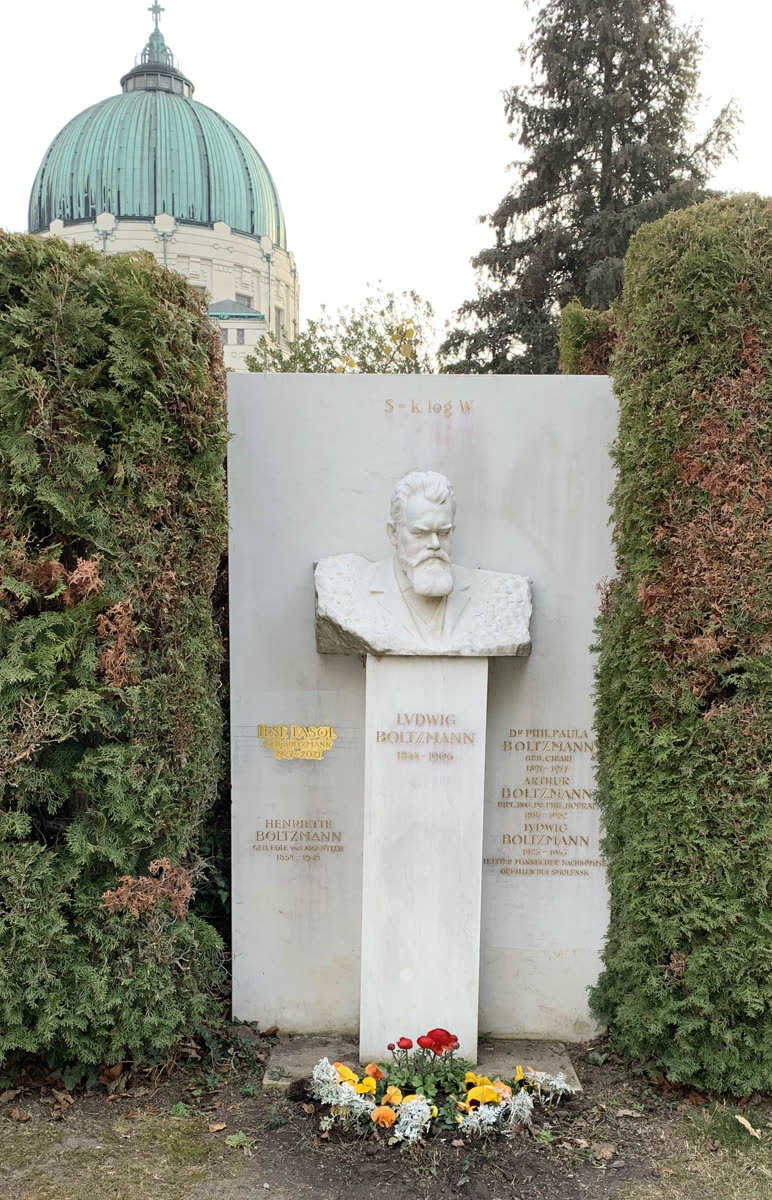
\includegraphics[width=\linewidth]{images/book4/boltzmann-grave.jpg}\par
{\footnotesize O túmulo de Boltzmann.}
\end{minipage}
\end{history}

\section{Exercícios}

\begin{exercise}[$\star$]\label{exo:b3:partition-functions:1}
Quatro osciladores compartilham quatro quanta. Liste as distribuições, dê o peso
de cada uma e verifique que eles somam o número de maneiras de colocar quatro
quanta \omterm{def:b3:many-electron-atoms:indistinguishable}{indistinguíveis} em quatro osciladores, $\binom{7}{3}$. Quais distribuições
são as mais prováveis?
\end{exercise}

\begin{exercise}[$\star$]\label{exo:b3:partition-functions:2}
Dois níveis não degenerados estão separados por \qty{2.5}{kJ/mol}. Calcule a razão
de suas \omterm{def:b3:partition-functions:boltzmann}{populações} a \qty{298.15}{K} e a \qty{1000}{K}. Qual é o limite a
temperatura muito alta?
\end{exercise}

\begin{exercise}[$\star$]\label{exo:b3:partition-functions:3}
% ledger: aw:Ar
Calcule o \omterm{def:b3:partition-functions:thermal-wavelength}{comprimento de onda térmico} de um átomo de argônio a \qty{298.15}{K} e
sua função de partição translacional em um volume de \qty{1}{dm^3}.
\end{exercise}

\begin{exercise}[$\star$]\label{exo:b3:partition-functions:4}
% ledger: diat:N2.Be, diat:N2.ae, diat:HCl.Be, diat:HCl.ae
Com $B_0 = \qty{1.990}{cm^{-1}}$ (\ce{N2}) e \qty{10.440}{cm^{-1}} (\ce{H^{35}Cl}), calcule $\theta_{\mathrm R}$ e a
função de partição rotacional de alta temperatura de cada molécula a
\qty{298.15}{K}.
\end{exercise}

\begin{exercise}[$\star\star$]\label{exo:b3:partition-functions:5}
% ledger: diat:I2.we, diat:I2.wexe, diat:N2.we, diat:N2.wexe
Os números de onda fundamentais de \ce{I2} e de \ce{N2} são \qty{213.27}{cm^{-1}} e
\qty{2329.92}{cm^{-1}}. Calcule $\theta_{\mathrm V}$, $q^{\mathrm V}$ a \qty{298.15}{K} e a fração das moléculas
que não estão em $v = 0$.
\end{exercise}

\begin{exercise}[$\star\star$]\label{exo:b3:partition-functions:6}
% ledger: diat:NO.split, lev:Cl.2P1_2
Calcule a função de partição eletrônica a \qty{298.15}{K} do \ce{NO} (dois níveis
duplamente degenerados separados por \qty{119.73}{cm^{-1}}) e do átomo de cloro (nível
fundamental ${}^2P_{3/2}$, ${}^2P_{1/2}$ a \qty{882.35}{cm^{-1}}). Que fração das moléculas de \ce{NO}
está no nível superior? Para que valor tende $q^{\mathrm E}(\ce{NO})$ a alta temperatura?
\end{exercise}

\begin{exercise}[$\star\star$]\label{exo:b3:partition-functions:7}
A partir de $q^{\mathrm T} = V/\Lambda^3$, deduza a energia interna e a capacidade calorífica a
volume constante de um mol de gás ideal monoatômico, e avalie $U - U(0)$ a
\qty{298.15}{K}.
\end{exercise}

\begin{exercise}[$\star\star$]\label{exo:b3:partition-functions:8}
% ledger: aw:Ar, s0:Ar_g
Use a equação de Sackur--Tetrode para calcular a entropia molar padrão do
argônio a \qty{298.15}{K}; compare com o valor tabelado
\qty{154.846}{J.K^{-1}.mol^{-1}}. Quanto ela muda se a pressão for dividida por 10?
\end{exercise}

\begin{exercise}[$\star\star$]\label{exo:b3:partition-functions:9}
% ledger: diat:HCl.Be, diat:HCl.ae
Calcule a contribuição rotacional para a entropia molar padrão de
\ce{H^{35}Cl} a \qty{298.15}{K} ($\theta_{\mathrm R} = \qty{15.02}{K}$).
\end{exercise}

\begin{exercise}[$\star\star\star$]\label{exo:b3:partition-functions:10}
Tratando $J$ como contínuo, mostre que o nível rotacional mais povoado de uma
molécula linear fica perto de $J_{\max} = \sqrt{T/2\theta_{\mathrm R}} - \frac12$. Avalie-o para \ce{HCl}
($\theta_{\mathrm R} = \qty{15.02}{K}$) e \ce{CO} ($\theta_{\mathrm R} = \qty{2.766}{K}$) a \qty{300}{K}. Por que os dois
ramos de uma banda de infravermelho são mais intensos algumas raias longe do centro?
\end{exercise}

\begin{exercise}[$\star\star\star$]\label{exo:b3:partition-functions:11}
% ledger: diat:H2.Be, diat:H2.ae
A fórmula de Euler--Maclaurin dá $\sum_{J\ge0}f(J) \approx \int_0^\infty f(J)\dd J + \frac12f(0) -
\frac1{12}f'(0)$. Aplique-a a $f(J) = (2J+1)\eu^{-\theta J(J+1)/T}$ e mostre que $q^{\mathrm R} \approx T/\theta +
\frac13$. Para que temperaturas $T/\theta$ é correto a 1\,\%? É aceitável para o \ce{H2}
($B_0 = \qty{59.32}{cm^{-1}}$) a \qty{298.15}{K}?
\end{exercise}

\begin{exercise}[$\star\star\star$]\label{exo:b3:partition-functions:12}
% ledger: diat:I2.we, diat:I2.wexe
Mostre que a entropia molar vibracional tende a zero quando $T \ll \theta_{\mathrm V}$ e a
$R[1 + \ln(T/\theta_{\mathrm V})]$ quando $T \gg \theta_{\mathrm V}$. Avalie a expressão exata e esse limite
para \ce{I2} ($\theta_{\mathrm V} = \qty{306.9}{K}$) a \qty{298.15}{K}, e comente.
\end{exercise}

\section{Problema: Contando a entropia do nitrogênio}

\begin{problem}[{Problema de fim de semana --- contando a entropia do nitrogênio: as
contribuições translacional, rotacional, vibracional e eletrônica para sua
entropia padrão, calculadas a partir de seu espectro e comparadas com a tabela}]
\label{pb:b3:partition-functions:1}
% ledger: aw:N, diat:N2.Be, diat:N2.ae, diat:N2.we, diat:N2.wexe, s0:N2_g, const:h, const:kB, const:NA, const:c
O nitrogênio é o principal gás do ar. Sua entropia molar padrão a
\qty{298.15}{K} é calculada aqui a partir de sua massa molar, \qty{28.014}{g/mol}, e de suas
constantes espectroscópicas: $B_e = \qty{1.998241}{cm^{-1}}$, $\alpha_e = \qty{0.017318}{cm^{-1}}$, $\omega_e =
\qty{2358.57}{cm^{-1}}$, $\omega_ex_e = \qty{14.324}{cm^{-1}}$; seu termo eletrônico fundamental é ${}^1\Sigma_g^+$.
Pressão padrão $p^\circ = \qty{1}{bar}$; $k = \qty{1.380649e-23}{J/K}$, $h = \qty{6.62607015e-34}{J.s}$.

\medskip\noindent\textbf{Parte I --- Translação.}
\begin{enumerate}
  \item Calcule a massa de uma molécula.
  \item Calcule seu \omterm{def:b3:partition-functions:thermal-wavelength}{comprimento de onda térmico} a \qty{298.15}{K}.
  \item Calcule o volume disponível por molécula, $kT/p^\circ$.
  \item Deduza $q^{\mathrm T}/N$ e comente seu tamanho.
  \item Calcule a entropia molar translacional.
  \item Quanto ela mudaria à metade da pressão?
\end{enumerate}

\medskip\noindent\textbf{Parte II --- Rotação.}
\begin{enumerate}[resume]
  \item Calcule $B_0$.
  \item Calcule $\theta_{\mathrm R}$.
  \item Dê o \omterm{def:b3:partition-functions:symmetry-number}{número de simetria} e diga o que ele leva em conta.
  \item Calcule $q^{\mathrm R}$ a \qty{298.15}{K}.
  \item A forma de alta temperatura é justificada?
  \item Calcule a entropia molar rotacional.
  \item Ignorando os pesos de spin nuclear, qual nível rotacional é o mais
        povoado?
\end{enumerate}

\medskip\noindent\textbf{Parte III --- Vibração e estados eletrônicos.}
\begin{enumerate}[resume]
  \item Calcule o quantum vibracional $G(1) - G(0)$.
  \item Calcule $\theta_{\mathrm V}$.
  \item Calcule $q^{\mathrm V}$ a \qty{298.15}{K}.
  \item Que fração das moléculas está em $v = 1$?
  \item Calcule a entropia molar vibracional.
  \item Qual é a contribuição eletrônica? Por que os estados eletrônicos excitados
        podem ser ignorados?
\end{enumerate}

\medskip\noindent\textbf{Parte IV --- Soma e comparação.}
\begin{enumerate}[resume]
  \item Some as contribuições.
  \item Compare com o valor tabelado \qty{191.609}{J.K^{-1}.mol^{-1}}.
  \item Em que medidas se apoia o valor calorimétrico de uma tabela?
  \item Por que as tabelas podem deixar de fora o spin nuclear?
  \item Enuncie o resultado: a entropia molar padrão do nitrogênio a \qty{298.15}{K}
        calculada a partir de suas constantes espectroscópicas.
\end{enumerate}
\end{problem}
